%	SDR-WinnComm Conference submission LaTeX template
%	Created by Mike Seery, michael.seery@afit.edu
%	No copyright; free for use at SDR-WinnComm

\documentclass[letterpaper,10pt,twocolumn]{article} %'draft' and 'final' modes are functional
\usepackage[english]{babel}
\usepackage{graphicx}
\usepackage{amsmath}
\usepackage{float}

%BEGIN formatting for winncomm
	
    %margins
    \usepackage[top=1in, bottom=1in, left=0.625in, right=0.625in]{geometry}%0.625 accounts for 1/4" spacing between columns
    \setlength{\columnsep}{0.25in}
    
    %title
    \usepackage{titling}
    \pretitle{\noindent\begin{center}\large\bfseries\MakeUppercase}
	\posttitle{\end{center}\noindent}
    \setlength{\droptitle}{-4em}     % Eliminate the default vertical space
	\addtolength{\droptitle}{0.37in}   % Only a guess. Use this for adjustment
    
    %% abstract adjustment
    \usepackage{abstract}
    \renewcommand{\abstractnamefont}{\normalfont\fontsize{10}{12}\bfseries\MakeUppercase}
    \renewcommand{\abstracttextfont}{\normalfont\fontsize{10}{12}}
    \setlength{\absleftindent}{0pt}
    \setlength{\absrightindent}{0pt}
    \setlength{\absparindent}{0pt}
    \setlength{\absparsep}{0pt}
    
    %decimal after section numbers    
    \renewcommand\thesection{\arabic{section}.}
	\renewcommand\thesubsection{\thesection\arabic{subsection}.}
	\renewcommand\thesubsubsection{\thesubsection\arabic{subsection}.}
    
    %section header spacing
    \usepackage{titlesec}
    \titlespacing*{\section}{0pt}{12pt}{10pt}
    \titlespacing*{\subsection}{0pt}{12pt}{10pt}
    \titlespacing*{\subsubsection}{0pt}{12pt}{0pt}
    
    %section header font and alignment
    \titleformat{\section}{\center\normalfont\bfseries}{\thesection}{1em}{\MakeUppercase}
    \titleformat{\subsection}{\normalfont\bfseries}{\thesubsection}{1em}{}
    \titleformat{\subsubsection}{\normalfont\itshape}{\thesubsubsection}{1em}{}
    
    %document font (Times)
    \usepackage{tgtermes}
	\usepackage[T1]{fontenc}
    
	%captions
    \usepackage[small]{caption}%font size
	\floatstyle{plaintop}%tables on top
	\restylefloat{table}%tables on top
    
    %bibliography: remove "--- ---" for ibid.'s
    \makeatletter
    \def\bstctlcite{\@ifnextchar[{\@bstctlcite}{\@bstctlcite[@auxout]}}
    \def\@bstctlcite[#1]#2{\@bsphack
      \@for\@citeb:=#2\do{%
        \edef\@citeb{\expandafter\@firstofone\@citeb}%
        \if@filesw\immediate\write\csname #1\endcsname{\string\citation{\@citeb}}\fi}%
      \@esphack}
    \makeatother
    
%% END Winncomm formatting

% Title Page
\title{A Novel Spectrum Technique for Wideband Single Carrier Transmission}

%\title{Hardware Implementation of Gold's algorithm for Rendezvous in Adaptable FH Cognitive Radio Networks}

\usepackage{authblk}
\renewcommand\Authfont{\large}
\renewcommand\Affilfont{\large}
\author[1]{fred harris (fharris@mail.sdsu.edu)}
\author[1]{Xiaofei Chen (chenxiaofei\_sdsu@yahoo.com)}
\author[1]{Elettra Venosa (elettra.venosa@unina2.it)}
\author[2]{Zhongren Cao (zcao@isi.edu)}
\affil[1]{San Diego State University, San Diego, CA, USA}
\affil[2]{Information Sciences Institute, University of Southern California, Arlington, VA, USA}


\date{\vspace{-2em}}%Do not type the date here. This removes the date by inserting negative space.

\begin{document}
\bstctlcite{biblio:BSTcontrol}%for bibliography control citation

	\maketitle
    
    %this removes page numbers
    \thispagestyle{empty}
	\pagestyle{empty}
      
	\begin{abstract}		 
     \noindent	%template - leave this
The abstract should appear at the top of the left-hand column of text, two line spaces below the author/affiliation information. 
Leave two line spaces between the end of the abstract and the beginning of the main text. 
The abstract should be approximately 150 words set in Times Roman 10 pt., 6 lines per inch (12 pt. line spacing). 
All manuscripts must be in English, printed in black ink, and follow the formatting instructions given in these instructions.
	\bigskip	%template - leave this
	\end{abstract}    

\section{Introduction}    	

\section{Non-Maximally Decimated Filter Bank Architecture}

In this section, we review the architecture of NMDFB, which is composed of a pair of filter banks and an intermediate processing unit in between the pair, as shown in Fig.~\ref{fig:nmdfbarchitecture}. The filter bank on the left side in Fig. is call analysis filter bank (AFB) and the one on the right is called the synthesis filter bank (SFB). The composite response of AFB and SFB satisfies the perfect reconstruction (PR) property, i.e, the combined effect of AFB and SFB only introduces delay in the absence of the intermediate processing unit. Historically, PR filter banks have been proposed in several contexts, among which maximally decimated cosine modulated filter banks [8, 9] are the most popular choice in image coding communities. NMDFB is particularly useful for communications waveform signal processing due to several reasons. First, the aliasing management of NMDFB is simply [10, 11]. Second, the design of basic prototype filters is straightforward according to targeted system dynamic range. Third, NMDFB architecture supports runtime updates inside the processing unit, thus it is applicable to time-varying scenarios.

\begin{figure*}[htb]
\centering
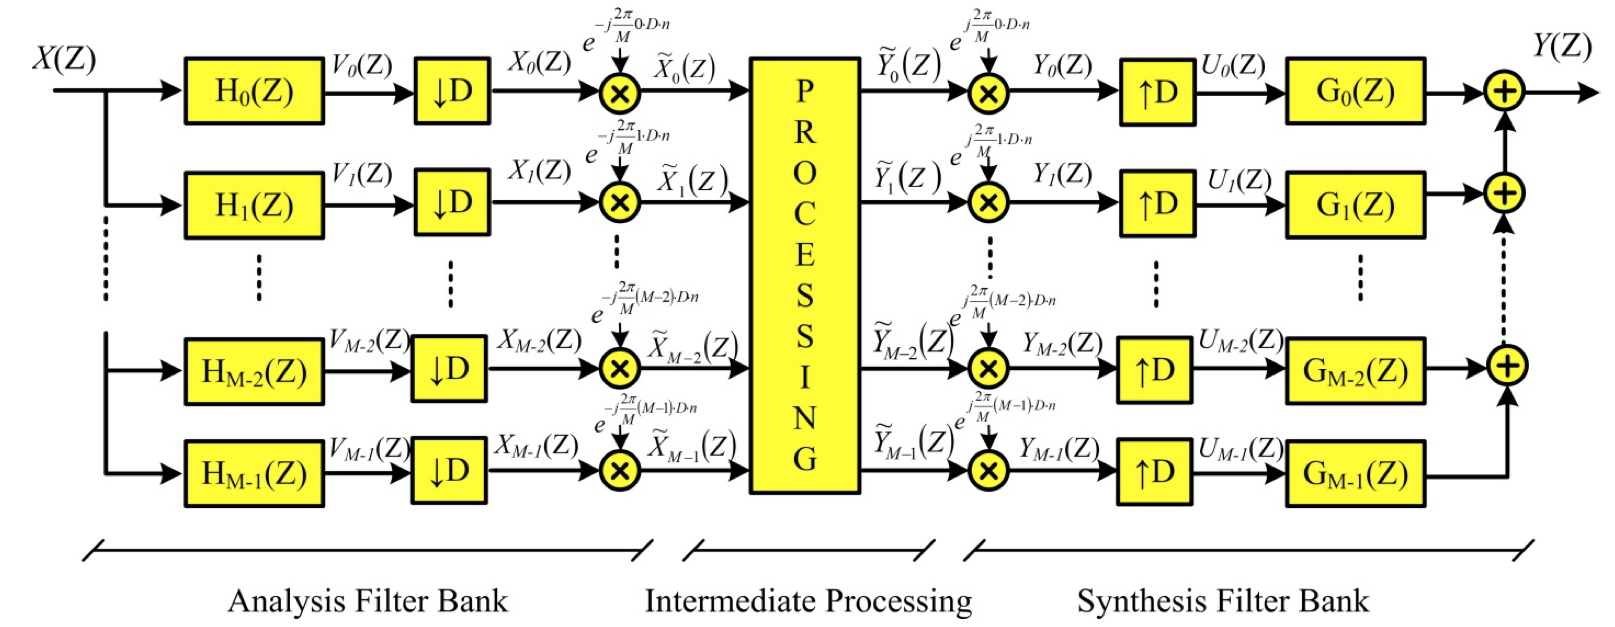
\includegraphics[width=\textwidth]{NMDFBArchitecture.png}
\caption{NMDFB architecture.}
\label{fig:nmdfbarchitecture}
\end{figure*}




\section{References}

 


%\todo[inline]{first line of each section is indented... fix it}

%\newpage
%
{\small
\bibliography{biblio}
% if `bib-example' is the name of
% your bib file
\bibliographystyle{IEEEtran}
% try changing to abbrvnat
}
    	
\end{document}